%//==============================--@--===========================//%
\clearpage
\subsection[5.6 WiFi: 802.11 Wireless LANs]{\hspace*{0.075 em}\raisebox{0.2 em}{$\pmb{\drsh}$} WiFi: 802.11 Wireless LANs}
\label{subsec:WLAN}

Wireless LANs (WLANs), particularly the IEEE 802.11 standard, have become ubiquitous in the modern world, providing internet access in various settings like homes, workplaces, and public areas. Despite having some physical layer differences, these standards share the 802.11 frame format, backward compatibility, and use the same medium access protocol, CSMA/CA. The 802.11ax standard also supports centralized scheduling.

{
\setlength{\tabcolsep}{8pt}

\begin{table}[h!]
    \centering
    \captionsetup{justification=centering}
    \begin{tabularx}{\textwidth}{lllll}
        \toprule
        IEEE 802.11 standard & Year & Max data rate & Range & Frequency\\
        \midrule
        802.11 n (WiFi 4) & $2009$ & $600$ Mbps & $70$ m & $2.4$, $5$ Ghz \\
        802.11 ac (WiFi 5) & $2013$ & $3.47$ Gpbs & $70$ m & $5$ Ghz \\
        802.11 ax (WiFi 6) & $2020$ (expected) & $14$ Gbps & $70$ m & $2.4$, $5$ Ghz \\
        \bottomrule
    \end{tabularx}
    \caption{Summary of some IEEE 802.11 standards \cite{Kurose2017}}
    \label{tab:WiFi-standards}
\end{table}
}

%//==============================--@--===========================//%
\vspace{-1.5 em}
\subsubsection[5.6.1 Wireless LAN Architecture]{$\rightarrow$ Wireless LAN Architecture}

The basic building block of the 802.11 architecture is the basic service set (BSS), comprising one or more wireless stations and an access point (AP). APs connect to interconnection devices, which in turn connect to the Internet. Each wireless station and AP have unique MAC addresses.

\vspace{-1.5 em}
\begin{figure}[ht] 
    \begin{subfigure}[b]{0.5\linewidth}%%
        \centering
        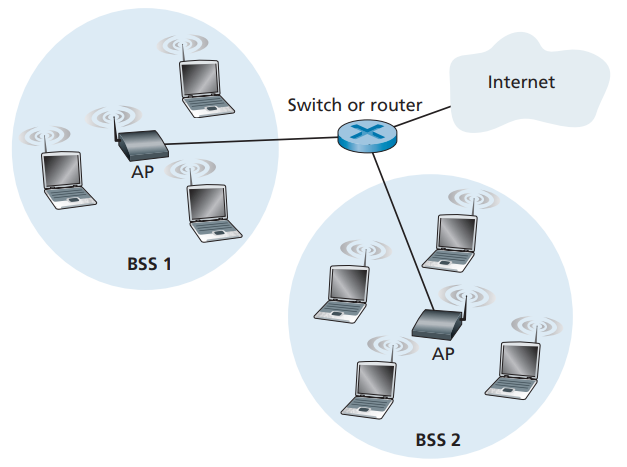
\includegraphics[width=0.8\linewidth]{img/5/rede-estruturada.png}
        \caption{Infrastructure wireless LAN (rede estruturada) \cite{Kurose2017}} 
        \label{fig:WiFi-net-a} 
    \end{subfigure}%% 
    \begin{subfigure}[b]{0.5\linewidth}
        \centering
        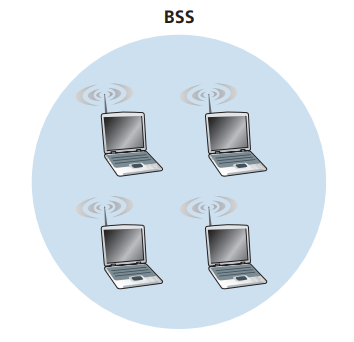
\includegraphics[width=0.8\linewidth]{img/5/rede-ad-hoc.png} 
        \caption{An ad hoc network \cite{Kurose2017}} 
        \label{fig:WiFi-net-b} 
    \end{subfigure}
    \caption{}
\end{figure}

\vspace{-1.5 em}
\begin{itemize}
    \item \textbf{Infrastructure wireless LANs} (\hyperref[fig:WiFi-net-b]{Fig. 62 (a)}):
    \begin{itemize}[noitemsep, nolistsep] \small
        \item Consist of wireless stations connected to an AP.
        \item AP connects to the wired network infrastructure.
        \item Centralized control, increased range, and access to wired resources.
        \item Stations associate with APs by passively or actively scanning channels.
        \item Device obtains IP address through DHCP.
    \end{itemize}

    \item \textbf{Ad hoc networks} (\hyperref[fig:WiFi-net-b]{Fig. 62 (b)}):
    \begin{itemize}[noitemsep, nolistsep] \small
        \item Decentralized networks without an AP.
        \item Wireless stations communicate directly with each other.
        \item Useful for temporary, spontaneous, or small-scale communication.
        \item Lacks centralized control and extended range of infrastructure networks.
    \end{itemize}
\end{itemize}

\renewcommand*{\thefootnote}{\fnsymbol{footnote}}
\footnotetext[4]{%
    Ad hoc networks do not inherently have direct access to the Internet. However, if one device in the network has an Internet connection (e.g., via cellular network or separate Wi-Fi), it can potentially share its connection with other devices through Internet Connection Sharing (ICS) or tethering, though performance may not be as robust as in infrastructure-based networks.
}
\renewcommand*{\thefootnote}{\arabic{footnote}}

%//==============================--@--===========================//%